%-----------------------------------------------------------------------------------------------%
%
% Maret 2019
% Template Latex untuk Tugas Akhir Program Studi Sistem informasi ini
% dikembangkan oleh Inggih Permana (inggihjava@gmail.com)
%
% Template ini dikembangkan dari template yang dibuat oleh Andreas Febrian (Fasilkom UI 2003).
%
% Orang yang cerdas adalah orang yang paling banyak mengingat kematian.
%
%-----------------------------------------------------------------------------------------------%

%-----------------------------------------------------------------------------%
\chapter{\babDua}
%-----------------------------------------------------------------------------%

%-----------------------------------------------------------------------------%

%-----------------------------------------------------------------------------%
\section{Profil Instansi}
\begin{longtable}{lll}
	Perguruan Tinggi                   & : & UIN Suska Riau                                                                                \\
	\endfirsthead
	%
	\multicolumn{3}{c}%
	{{\bfseries Lanjutan dari halaman sebelumnya}}                                                                                         \\
	Perguruan Tinggi                   & : & UIN Suska Riau                                                                                \\
	\endhead
	%
	Fakultas                           & : & Sains dan Teknologi                                                                           \\
	Program Studi                      & : & Sistem Informasi                                                                              \\
	Jenjang                            & : & Strata 1 (S1)                                                                                 \\
	No. SK Pendirian Program Studi     & : & DJ.II/26/2006                                                                                 \\
	SK Penyelenggaraan                 & : & 3480/D/T/K-AI/2009                                                                            \\
	Tanggal SK Pendirian Program Studi & : & 20 Februari 2006                                                                              \\
	Pejabat Penandatangan SK           & : & Direktur Jenderal Perguruan Tinggi                                                            \\
	Penyelenggaraan Program Studi      & : & Juli 2002                                                                                     \\
	Nomor SK Izin Operasional          & : & Dj.I/123/2012                                                                                 \\
	Tanggal SK Izin Operasional        & : & 25 Januari 2012                                                                               \\
	Akreditasi Program Studi           & : & Baik Sekali                                                                                   \\
	Keberlakuan Akreditasi             & : & 19 Maret 2024 - 19 Maret 2029                                                                 \\
	Nomor SK LAM INFOKOM               & : & 018/SK/LAM-INFOKOM/Ak/S/III/2024                                                              \\
	Email                              & : & faste.sif@uin-suska.ac.id                                                                     \\
	Website                            & : & https://sif.uin-suska.ac.id/                                                                  \\
	Alamat                             & : & \begin{tabular}[c]{@{}l@{}}Jl. HR. Soebrantas No. 155 KM 15, \\ Pekanbaru 28293.\end{tabular}
\end{longtable}
%-----------------------------------------------------------------------------%
\subsection{Sejarah}
%-----------------------------------------------------------------------------%
UIN Suska Riau memiliki fasilitas infrastruktur pendukung Tridharma Perguruan Tinggi yang baik, salah satunya adalah laboratorium terpadu di bawah Fakultas Sains dan Teknologi yang dikelola oleh Program Studi Sistem Informasi sejak tahun 2002. Terdapat tiga laboratorium yang dikelola oleh Program Studi Sistem Informasi, yaitu Laboratorium Rekayasa Sistem Informasi (RSI), Laboratorium Internet (INT), dan Laboratorium \textit{Software Engineering} (SE). Ketiga laboratorium tersebut merupakan aset penting yang dapat dimanfaatkan dengan baik untuk mencapai target-target universitas dan menghasilkan lulusan Program Studi Sistem Informasi yang kompeten dalam pendidikan, penelitian, serta pengabdian masyarakat dengan mengintegrasikan nilai-nilai keislaman. Laboratorium-laboratorium tersebut tidak hanya digunakan untuk praktikum mahasiswa sesuai dengan kurikulum, tetapi juga mampu mendukung berbagai kegiatan mahasiswa dan dosen dalam meningkatkan pengetahuan di bidang Sistem Informasi.
% -----------------------------------------------------------------------------%
\subsection{Visi}
% -----------------------------------------------------------------------------%
Menjadi laboratorium Program Studi Sistem Informasi yang memiliki keunggulan dalam bidang pendidikan, penelitian, dan pengabdian kepada masyarakat dengan menghasilkan lulusan yang proaktif, inovatif, dan profesional dalam bidang Sistem Informasi di tingkat lokal, regional, dan nasional yang berbasis nilai-nilai islami pada tahun 2030.
% -----------------------------------------------------------------------------
\subsection{Misi}
% -----------------------------------------------------------------------------%
Untuk mencapai Visi Laboratorium Program Studi Sistem Informasi, berikut Misi-misi yang harus dicapai, diantaranya:

\begin{enumerate}

	\item Mendukung penyelenggaraan kegiatan pendidikan akademik dan praktikum berbasis teknologi kepada mahasiswa, dosen, dan stakeholder.
	\item Mendukung pelaksanaan kegiatan penelitian yang berbasis teknologi kepada mahasiswa, dosen, dan stakeholder.
	\item Mendukung kegiatan pengabdian kepada masyarakat yang berbasis teknologi.
	\item Menyiapkan sumber daya manusia yang mampu menerapkan teknologi informasi khususnya dibidang Sistem Informasi.
	\item Membangun kemitraan dan jejaring dengan industri, pemerintah, dan organisasi nasional.

\end{enumerate}
% -----------------------------------------------------------------------------%
\subsection{Struktur Organisasi}
% -----------------------------------------------------------------------------%
Untuk menjalankan Tridharma Perguruan Tinggi dengan baik, pengelola laboratorium harus memiliki kemampuan manajerial yang baik dan dibantu dengan keahlian IT. Untuk mencapai hal ini, diperlukan sekelompok pengelola laboratorium yang percaya diri dan memiliki kemampuan. Gambar 2.1 menunjukkan struktur organisasi pengelola laboratorium Program Studi Sistem Informasi dari 2021 hingga 2024.

\begin{figure}
	\centering
	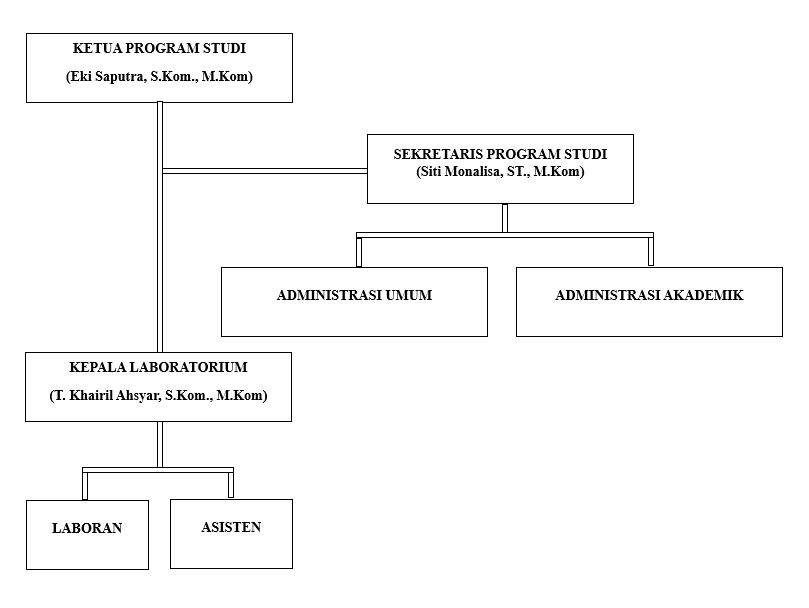
\includegraphics[width=0.82\linewidth]{konten/gambar/Struktur Organisasi.png}
	\caption{Struktur Organisasi Laboratorium \protect\cite{labsi2023}}
	\label{fig:struktur-organisasi}
\end{figure}

%-----------------------------------------------------------------------------%

\section{Pengembangan Sistem Informasi}
Pengembangan sistem mengacu pada proses terstruktur pembuatan dan pemeliharaan sistem informasi, yang mencakup perangkat keras, perangkat lunak, data, prosedur, dan personel. Proses ini sangat penting untuk mengatasi tantangan organisasi dan memanfaatkan peluang melalui implementasi sistem berbasis komputer \cite{efendi2023perkembangan}. Biasanya melibatkan beberapa tahap, termasuk perencanaan, analisis sistem, desain, pengembangan, pengujian, integrasi, dan pemeliharaan \cite{kiplie2018system}. Rekayasa sistem memainkan peran penting dalam konteks ini, karena menekankan pemahaman kebutuhan pelanggan dan mengelola sistem yang kompleks sepanjang siklus hidup mereka \cite{furterer2018applying}. Selain itu, aspek digitalisasi pengembangan sistem menyoroti pentingnya mengubah informasi nyata menjadi format elektronik, sehingga meningkatkan aksesibilitas dan pelestarian data kritis \cite{kiplie2018system}. Secara keseluruhan, pengembangan sistem yang efektif mengintegrasikan keahlian teknis dengan ketajaman bisnis untuk memastikan bahwa sistem memenuhi harapan pengguna dan tujuan organisasi \cite{ahmed2014developing}.

\section{Manajemen}
Manajemen didefinisikan sebagai proses perencanaan, pengorganisasian, memimpin, dan mengendalikan sumber daya untuk mencapai tujuan tertentu secara efisien dan efektif \cite{kaehler2019concept}. Definisi dasar ini menggarisbawahi pentingnya manajemen dalam berbagai konteks, termasuk olahraga dan bisnis, di mana ia memastikan realisasi tujuan operasional dan strategis \cite{kaehler2019concept}. Fungsi utama manajemen — perencanaan, pengorganisasian, kepemimpinan, dan pengendalian — sangat penting untuk kelancaran operasi organisasi manapun \cite{feng2009internal}. Selain itu, berbagai teori manajemen, seperti teori klasik dan perilaku, menyediakan kerangka kerja yang membantu manajer mengembangkan strategi efektif yang disesuaikan dengan lingkungan unik mereka \cite{hussain2019management}. Pada akhirnya, manajemen strategis mencakup perumusan dan implementasi tujuan utama, dengan mempertimbangkan faktor internal dan eksternal, yang sangat penting untuk kesuksesan jangka panjang dan keunggulan kompetitif \cite{schuhly2022strategic}.

\section{Manajemen Laboratorium}
Manajemen laboratorium mencakup pendekatan sistematis untuk mengawasi operasi laboratorium, yang mencakup pengumpulan data, manajemen inventaris, dan memastikan kontrol kualitas. Ini melibatkan integrasi berbagai komponen seperti tenaga kerja, peralatan, dan sumber daya keuangan untuk meningkatkan efisiensi operasional dan mendukung inovasi ilmiah \cite{marwah2024sistem}. Sistem manajemen laboratorium modern telah berkembang untuk memasukkan solusi digital yang mengotomatiskan proses, meningkatkan aksesibilitas data, dan memfasilitasi berbagi sumber daya, sehingga mengatasi keterbatasan metode tradisional \cite{rihm2024digital}. Aspek kunci dari manajemen laboratorium yang efektif juga melibatkan praktik penjaminan kualitas, yang memastikan kepatuhan terhadap praktik laboratorium yang baik dan keandalan hasilnya \cite{kawai2021phase}. Secara keseluruhan, manajemen laboratorium yang efektif sangat penting untuk mengoptimalkan fungsi laboratorium, meningkatkan hasil pendidikan, dan mendorong kemajuan ilmiah \cite{marwah2024sistem}.

\section{Laboratorium}
Laboratorium merupakan sarana dalam melaksanakan sebuah riset dalam bidang ilmiah, eksperimen, pengukuran maupun pelatihan ilmiah. Meski laboratorium telah memiliki alat-alat yang lengkap, pengelolaan laboratorium juga harus diperhatikan. Adanya alat-alat yang sudah lengkap dan penggunaan yang sudah baik tentunya perlu untuk dilakukan manajemen yang baik pada laboratorium tersebut, karena terdapat beberapa hal yang harus diperhatikan kembali seperti pengelolaan masing-masing laboratorium dan pengolahan data \cite{sweden2022rancang}.

\subsection{Laboratorium Rekayasa Sistem Informasi (RSI)}
Laboratorium Rekayasa sistem Informasi atau yang disingkat dengan nama Laboratorium RSI merupakan laboratorium pertama yang dimiliki oleh Program Studi Sistem Informasi sejak pindahnya aktivitas perkuliahan kampus dari kampus Sukajadi ke kampus utama Panam Pekanbaru Riau pada tahun 2007. Fungsi utama dari laboratorium ini adalah sebagai fasilitas infrastruktur pendukung untuk pelaksanaan kegiatan perkuliahan praktikum bagi mahasiswa Program Studi Sistem Informasi terkait bidang Rekayasa Sistem Informasi. Bidang Rekayasa Sistem Informasi merupakan bidang yang paling dominan yang ada di Program Studi Sistem Informasi \cite{lab-si-website}.

\begin{figure}
	\centering
	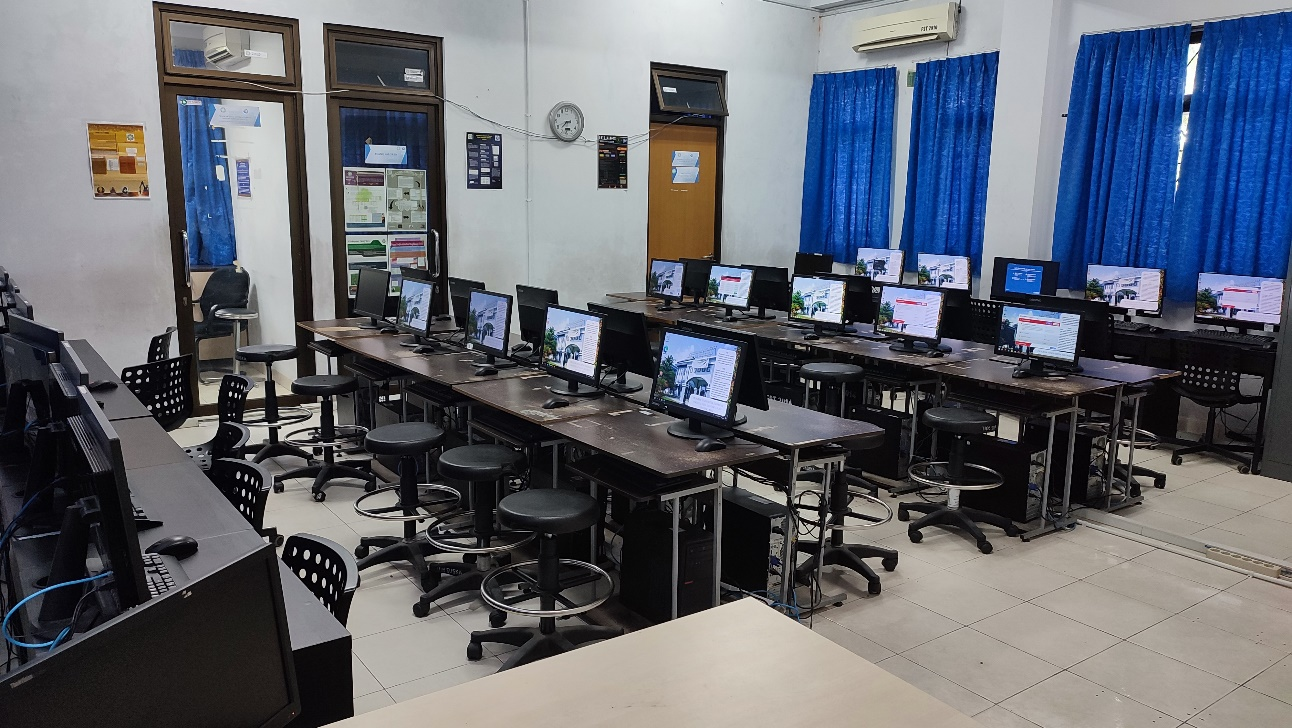
\includegraphics[width=0.82\linewidth]{konten/gambar/lab-rsi.jpg}
	\caption{Laboratorium Rekayasa Sistem Informasi \protect\cite{labsi2023}}
	\label{fig:lab-rsi}
\end{figure}

\subsection{Laboratorium Internet (INT)}
Laboratorium Internet atau yang disingkat dengan nama Laboratorium INT merupakan laboratorium milik Program Studi Sistem Informasi di bawah Fakultas Sains dan Teknologi kedua yang aktivitas perkuliahannya berada di kampus utama Panam Pekanbaru Riau. Secara spesifik, laboratorium ini lebih dioperasikan untuk kebutuhan perkuliahan terkait matakuliah praktikum dasar, seperti matakuliah Jaringan Komputer dan Pemrograman Dasar \cite{lab-si-website}.

\begin{figure}
	\centering
	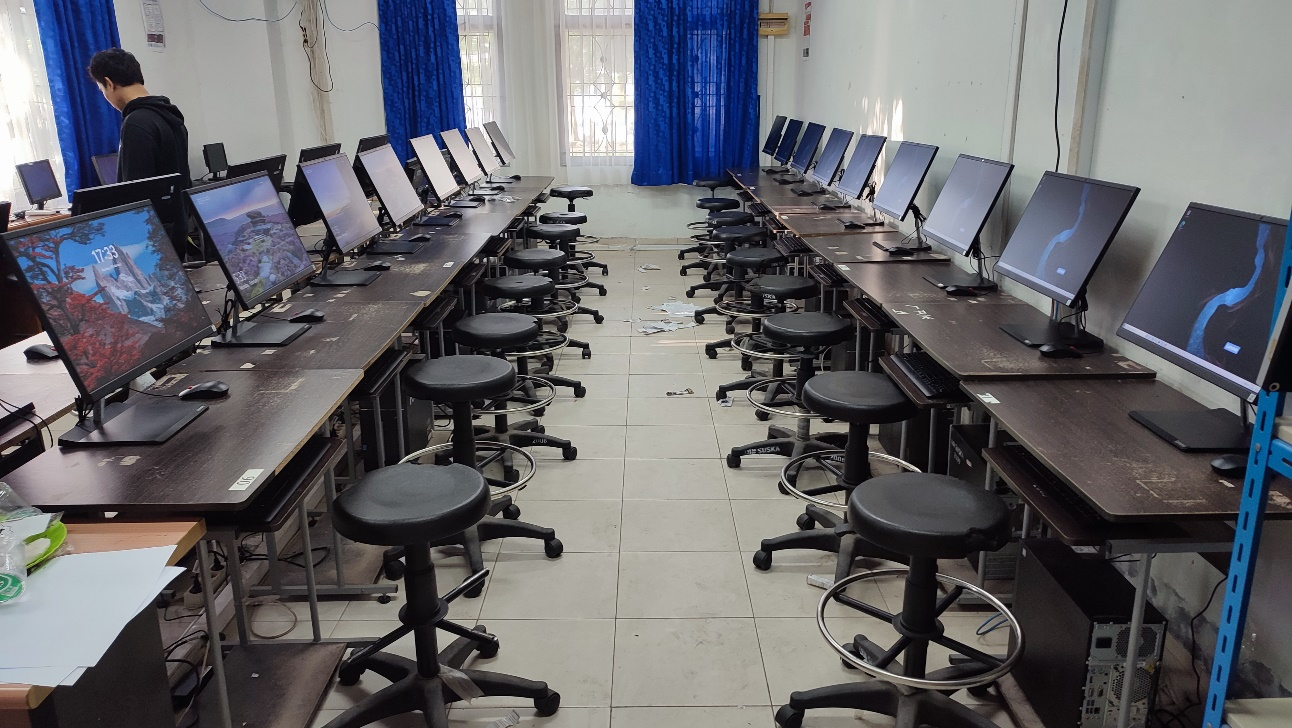
\includegraphics[width=0.82\linewidth]{konten/gambar/lab-internet.jpg}
	\caption{Laboratorium Internet \protect\cite{labsi2023}}
	\label{fig:lab-int}
\end{figure}

\subsection{Laboratorium \textit{Software Engineering} (SE)}
Laboratorium ke tiga yang dimiliki oleh Program Studi Sistem Informasi adalah Laboratorium \textit{Software Engineering} atau yang disingkat dengan nama Laboratorium SE. Laboratorium ini merupakan laboratorium terbaru milik yang dikelola oleh Program Studi dari usulan pengadaan barang tahun anggaran 2021 di bawah naungan Fakultas Sains dan Teknologi UIN Suska Riau. Adapun laboratorium SE sebagai pendukung dalam pelaksanaan kegiatan perkuliahan praktikum bagi mahasiswa Program Studi Sistem Informasi yang terkait dengan bidang keilmuan seperti Praktikum Basis Data, Pemrograman Beorientasi Objek (PBO), dan matakuliah wajib praktikum lainnya \cite{lab-si-website}.

\begin{figure}
	\centering
	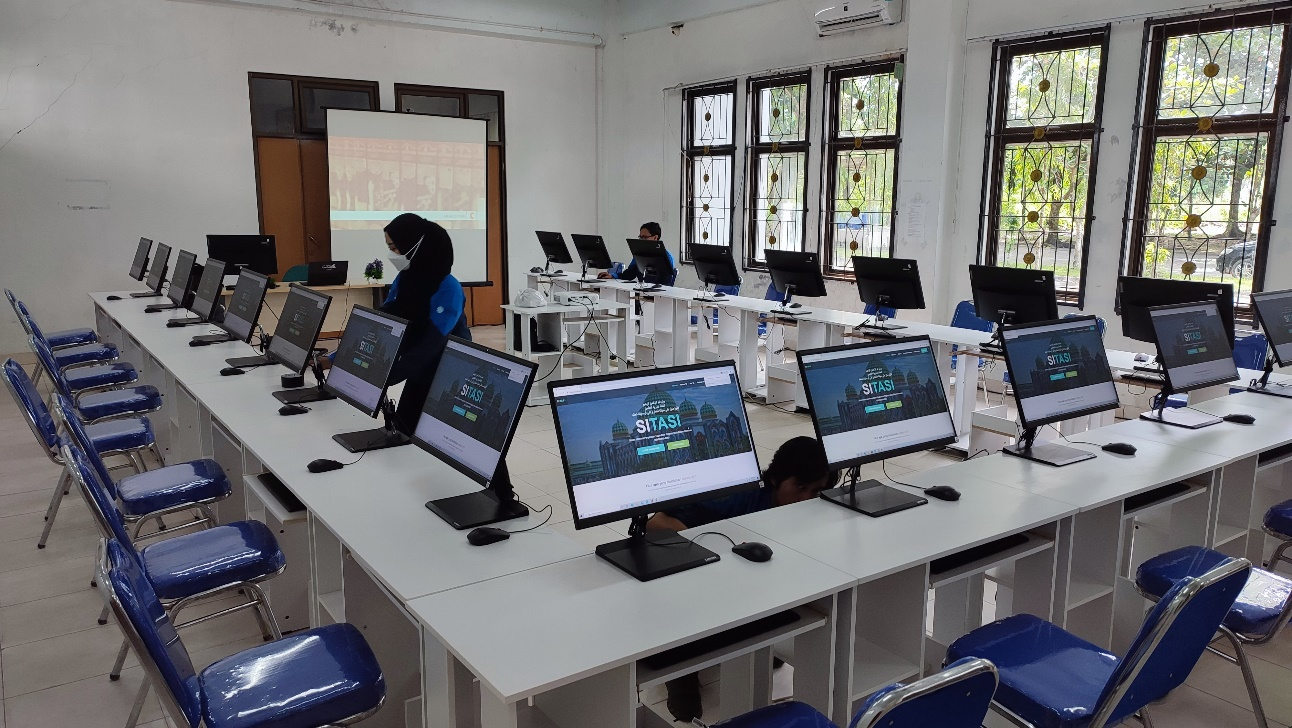
\includegraphics[width=0.82\linewidth]{konten/gambar/lab-se.jpg}
	\caption{Laboratorium \textit{Software Engineering} \protect\cite{labsi2023}}
	\label{fig:lab-se}
\end{figure}

\section{SITASI}
SITASI adalah sebuah sistem yang dirancang khusus untuk pengelolaan Tugas Akhir Program Studi Sistem Informasi UIN Sultan Syarif Kasim Riau. Pengembangan sistem ini dilakukan oleh mahasiswa dengan prinsip “Dari mahasiswa, Oleh mahasiswa, dan Untuk mahasiswa“. “Dari mahasiswa” maksudnya adalah ide-ide dari fitur-fitur yang ada pada SITASI berasal dari mahasiswa. “Oleh mahasiswa” maksudnya adalah implementasi dari ide-ide tersebut dilakukan oleh mahasiswa. Sedangkan “Untuk mahasiswa”, SITASI ini memang bertujuan untuk mahasiswa. Selain itu SITASI telah menjadi tempat belajar pengembangan sistem informasi bagi mahasiswa Program Studi Sistem Informasi. Link : https://sitasi.uin-suska.ac.id \cite{web-prodi}.

\begin{figure}
	\centering
	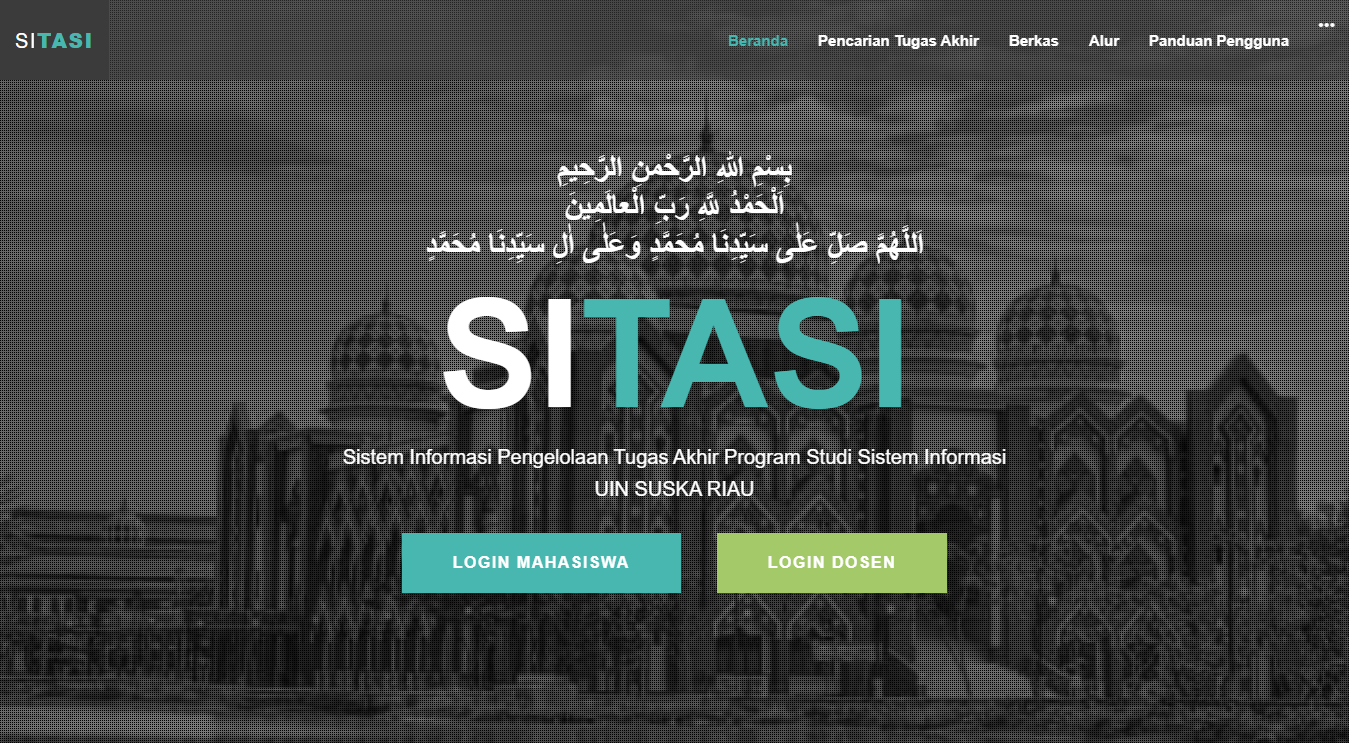
\includegraphics[width=0.82\linewidth]{konten//gambar/sitasi.png}
	\caption{Sistem Informasi Tugas Akhir \protect\cite{web-prodi}}
	\label{fig:enter-label}
\end{figure}

\section{SmarTA}
SmarTA ini merupakan aplikasi yang digunakan untuk mendeteksi Gambar yang tidak dirujuk, Tabel yang tidak dirujuk, Persamaan/Rumus yang tidak dirujuk, Lampiran yang tidak dirujuk, Label Gambar dan Label Tabel yang sama, dan kesalahan format penulisan tanda baca, serta tabel dengan format Non-LongTable. Aplikasi ini dibangun, mengingat masih banyak kesalahan-kesalahan penulisan yang terdapat pada laporan akhir mahasiswa pada saat ingin melakukan validasi atau jilid keras Laporan TA. Sistem ini dapat mengurangi pekerjaan dosen pembimbing maupun koordinator TA dalam mendeteksi kesalahan-kesalahan penulisan agar dapat menjaga kualitas Laporan Tugas Akhir dari sisi penulisan \cite{web-prodi}.

\begin{figure}
	\centering
	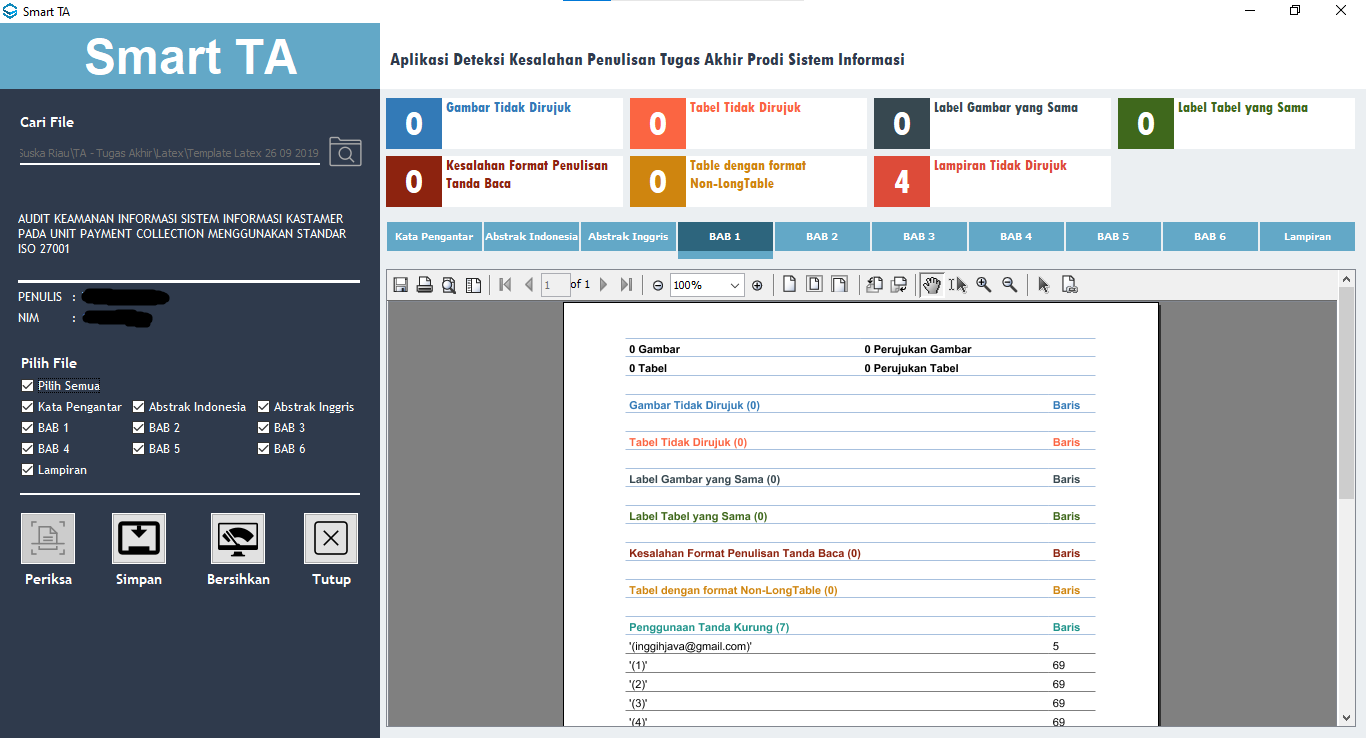
\includegraphics[width=0.82\linewidth]{konten//gambar/smartta.png}
	\caption{Sistem Pengecekan Penulisan Tugas Akhir \protect\cite{web-prodi}}
	\label{fig:enter-label}
\end{figure}

\section{SIKAPE}
Sistem Kerja Praktek ini atau yang disingkat dengan SIKAPE merupakan sistem yang digunakan untuk manajemen dan administrasi Kerja Praktek yang dikelola oleh Program Studi Sistem Informasi. Target dari sistem ini agar mempermudah jalannya proses Kerja Praktek yang dilakukan oleh mahasiswa Program Studi Sistem Informasi UIN Suska Riau. Sistem ini diharapkan dapat memangkas alur proses Kerja Praktek yang selama ini masih dilakukan secara manual. Saat ini, sistem ini rencananya akan diintegrasikan dengan Sistem Informasi Tugas Akhir (SITASI) agar lebih efektif dalam pengembangan berikutnya \cite{web-prodi}.

\begin{figure}
	\centering
	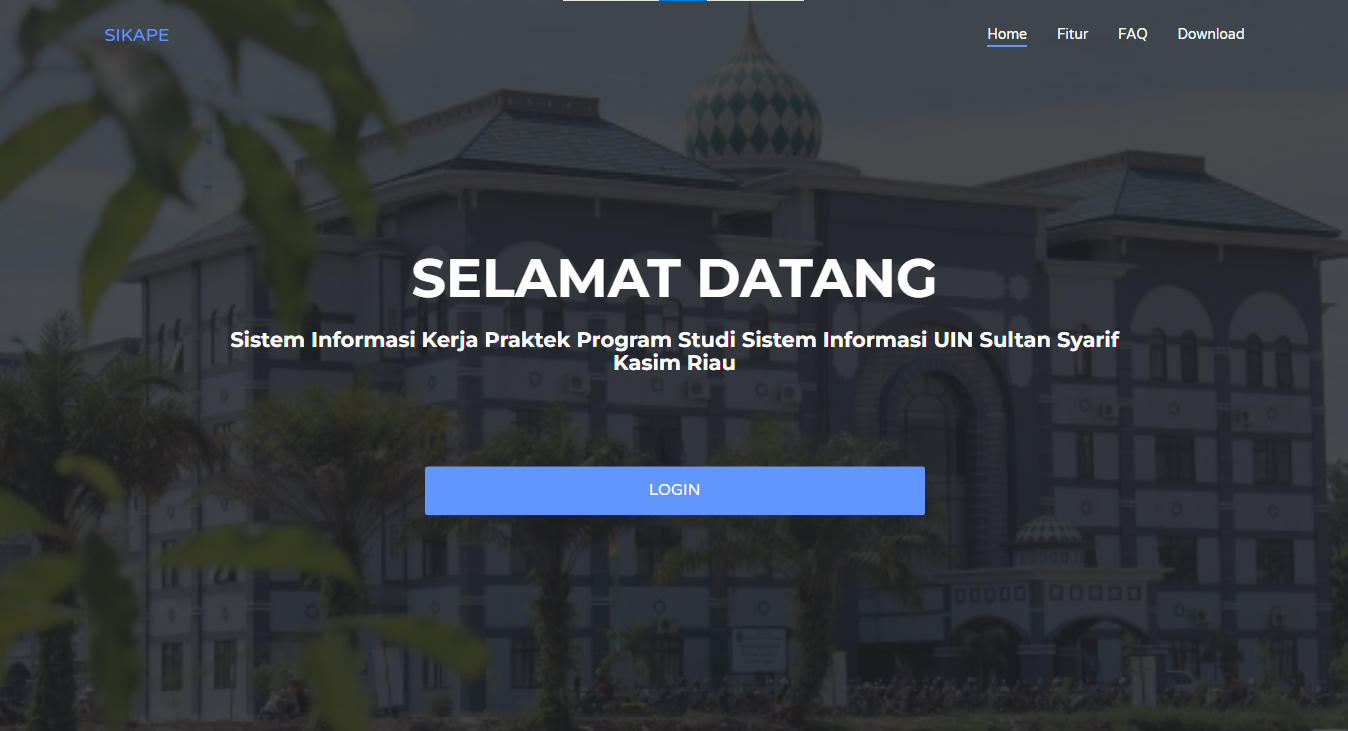
\includegraphics[width=0.82\linewidth]{konten//gambar/sikape.png}
	\caption{Sistem Kerja Praktek \protect\cite{web-prodi}}
	\label{fig:enter-label}
\end{figure}

\section{SIREPO}
Sistem ini dibangun untuk menyimpan dokumen-dokumen khusus terkait hasil penelitian, Tugas Akhir, dan Kerja Praktek mahasiswa Program Studi Sistem Informasi dalam bentuk project, serta untuk menyimpan dan menyelamatkan dokumen-dokumen penting laboratorium secara digitalisasi. Mengingat keterbatasan dan keamanan ruang penyimpanan laboratorium, oleh sebab itu di bangunlah Sistem Repositori yang disingkat SIREPO. Untuk project ini, sistem yang dibangun lebih bersifat custom software opensource yang disesuaikan dengan kebutuhan laboratorium. Mahasiswa diajarkan bagaimana mengelola dokumen-dokumen penting yang harus diselematkan untuk jangka waktu yang lama dalam mendukung pengelolaan Program Studi Sistem Informasi khususnya laboratorium yang berbasis IT. Link : https://repo.lab-si.uin-suska.ac.id \cite{web-prodi}.

\begin{figure}
	\centering
	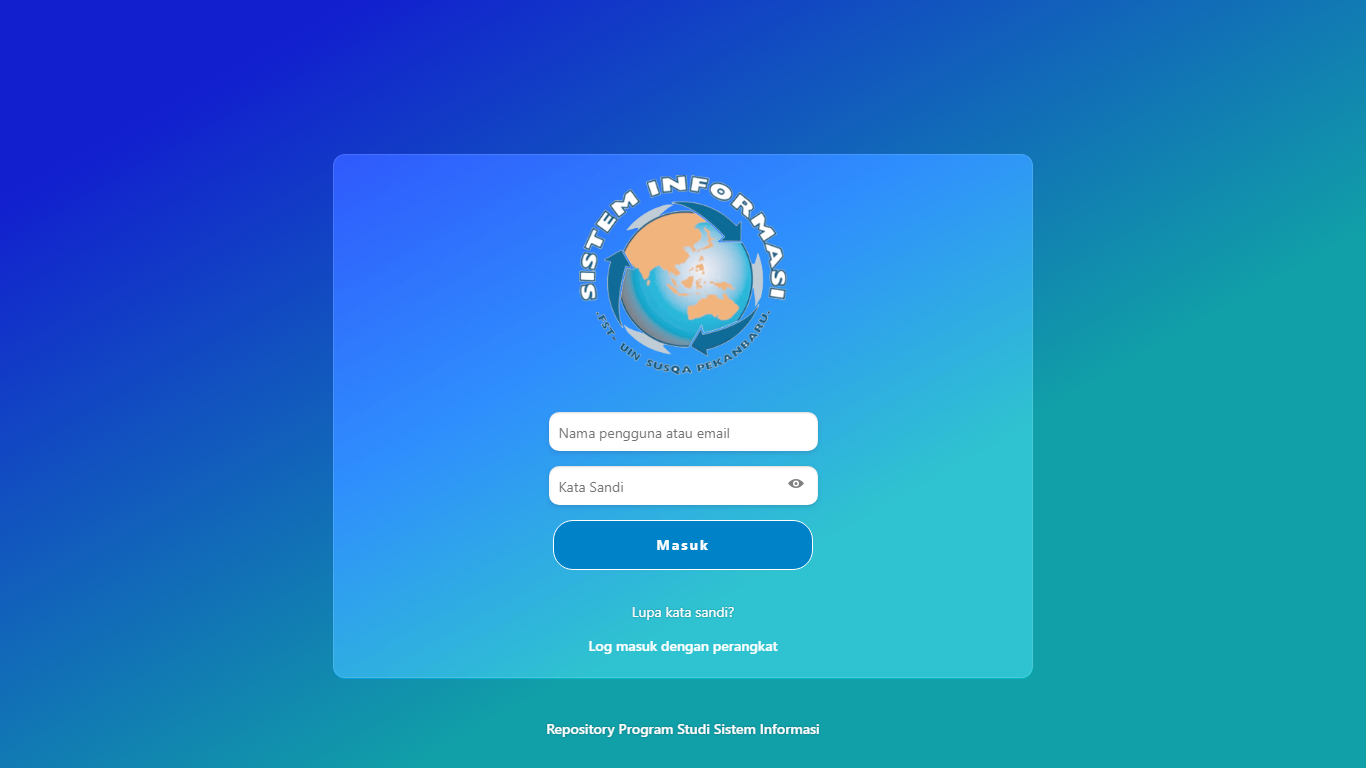
\includegraphics[width=0.82\linewidth]{konten//gambar/sirepo.png}
	\caption{\textit{Repository} Laboratorium \protect\cite{web-prodi}}
	\label{fig:enter-label}
\end{figure}

\section{Lab SI \textit{Website}}
Seiring dengan bertambah banyaknya informasi yang perlu disampaikan ke publik mengenai keberadaan (eksistensi) Laboratorium Program Studi Sistem Informasi, maka diperlukan media publik yang dapat menyampaikan informasi sekaligus promosi fasilitas dan layanan kepada khalayak umum mengenai keberadaan Laboratorium yang dimiliki oleh Program Studi Sistem Informasi Fakultas Sains dan Teknologi UIN Sultan Syarif Kasim Riau. Website ini dibangun untuk dapat meng-cover hal-hal yang bersifat informasi agar pihak-pihak luar dapat mengetahui lebih mendalam tentang profil Program Studi \cite{kusuma2024penerapan}. Hal ini juga memberikan peluang kepada pihak luar yang ingin bekerja sama dengan memanfaatkan fasilitas laboratorium program studi untuk kegiatan-kegiatan akademik dan non akademik.  Link Website Laboratorium : https://lab-si.uin-suska.ac.id \cite{web-prodi}.

\begin{figure}
	\centering
	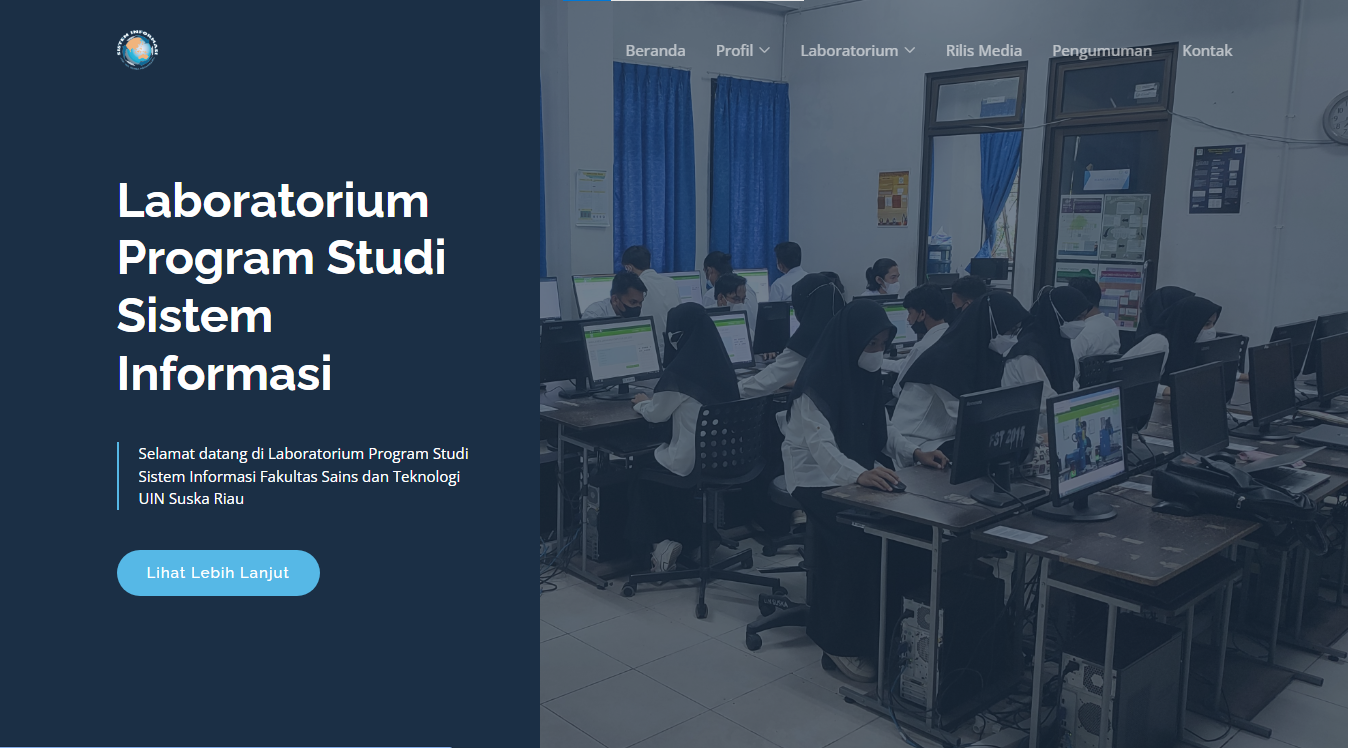
\includegraphics[width=0.82\linewidth]{konten//gambar/labsi.png}
	\caption{Website Laboratorium Program Studi Sistem Informasi \protect\cite{web-prodi}}
	\label{fig:enter-label}
\end{figure}

\section{LABVIS}
LABVIS adalah sistem yang dirancang untuk mengelola dan memantau aktivitas kunjungan di laboratorium komputer Prodi Sistem Informasi. Dengan memanfaatkan scan QR Code pada kartu kunjungan, pengunjung dapat secara praktis mencatat riwayat kehadirannya. Grafik kunjungan interaktif memberikan visualisasi yang jelas tentang tren kunjungan mingguan, bulanan, dan tahunan. Terlebih lagi, LABVIS mampu menyimpan riwayat kunjungan untuk setiap pengunjung, memungkinkan mereka untuk terlacak di setiap kali aktivitasnya di laboratorium. Dengan begitu, LABVIS secara efektif berperan dalam melindungi lingkungan laboratorium agar dapat terjaga dengan baik \cite{web-prodi}.

\begin{figure}
	\centering
	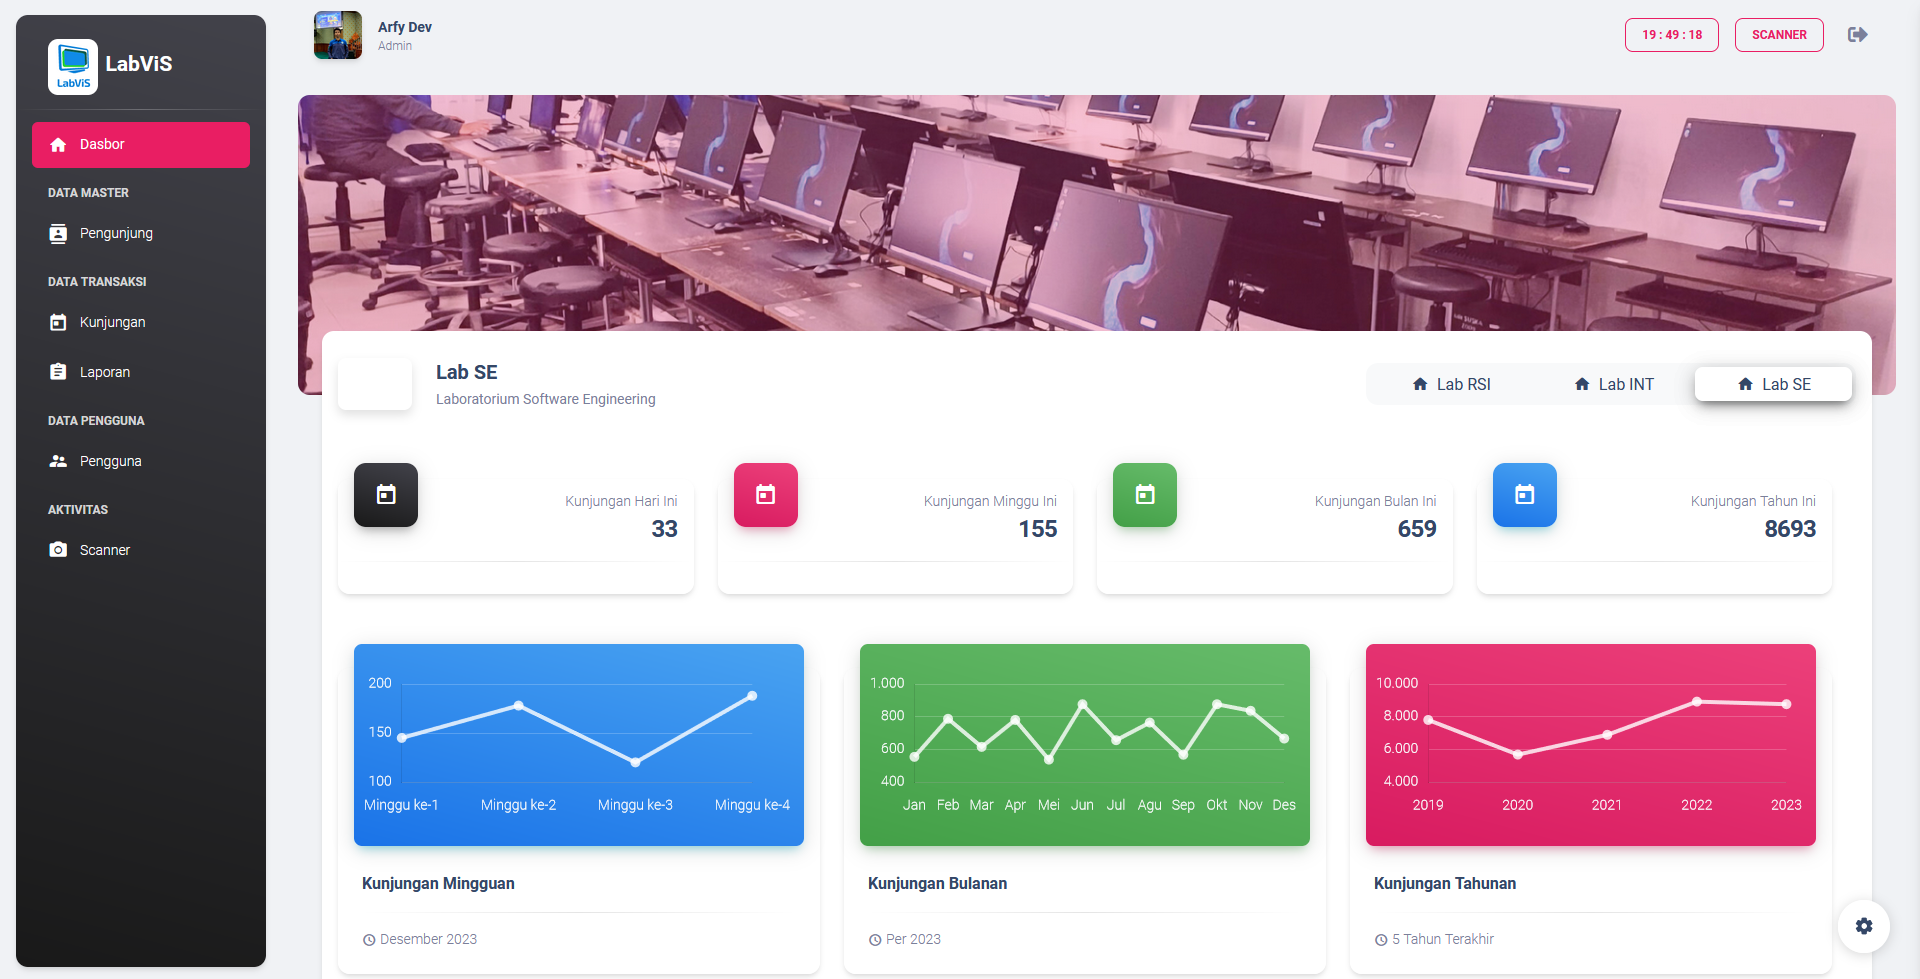
\includegraphics[width=0.82\linewidth]{konten//gambar/labvis.png}
	\caption{\textit{Laboratory Visitor System (LABVIS)} \protect\cite{web-prodi}}
	\label{fig:labvis}
\end{figure}

\section{LARIS}
LARIS adalah sistem pendaftaran dan pengelolaan asisten laboratorium. Sistem ini digunakan untuk mengelola asisten laboratorium program studi sistem informasi mulai dari tahan pendaftaran, rekrutmen, hingga menjadi asisten laboratorium \cite{web-prodi}.

\begin{figure}
	\centering
	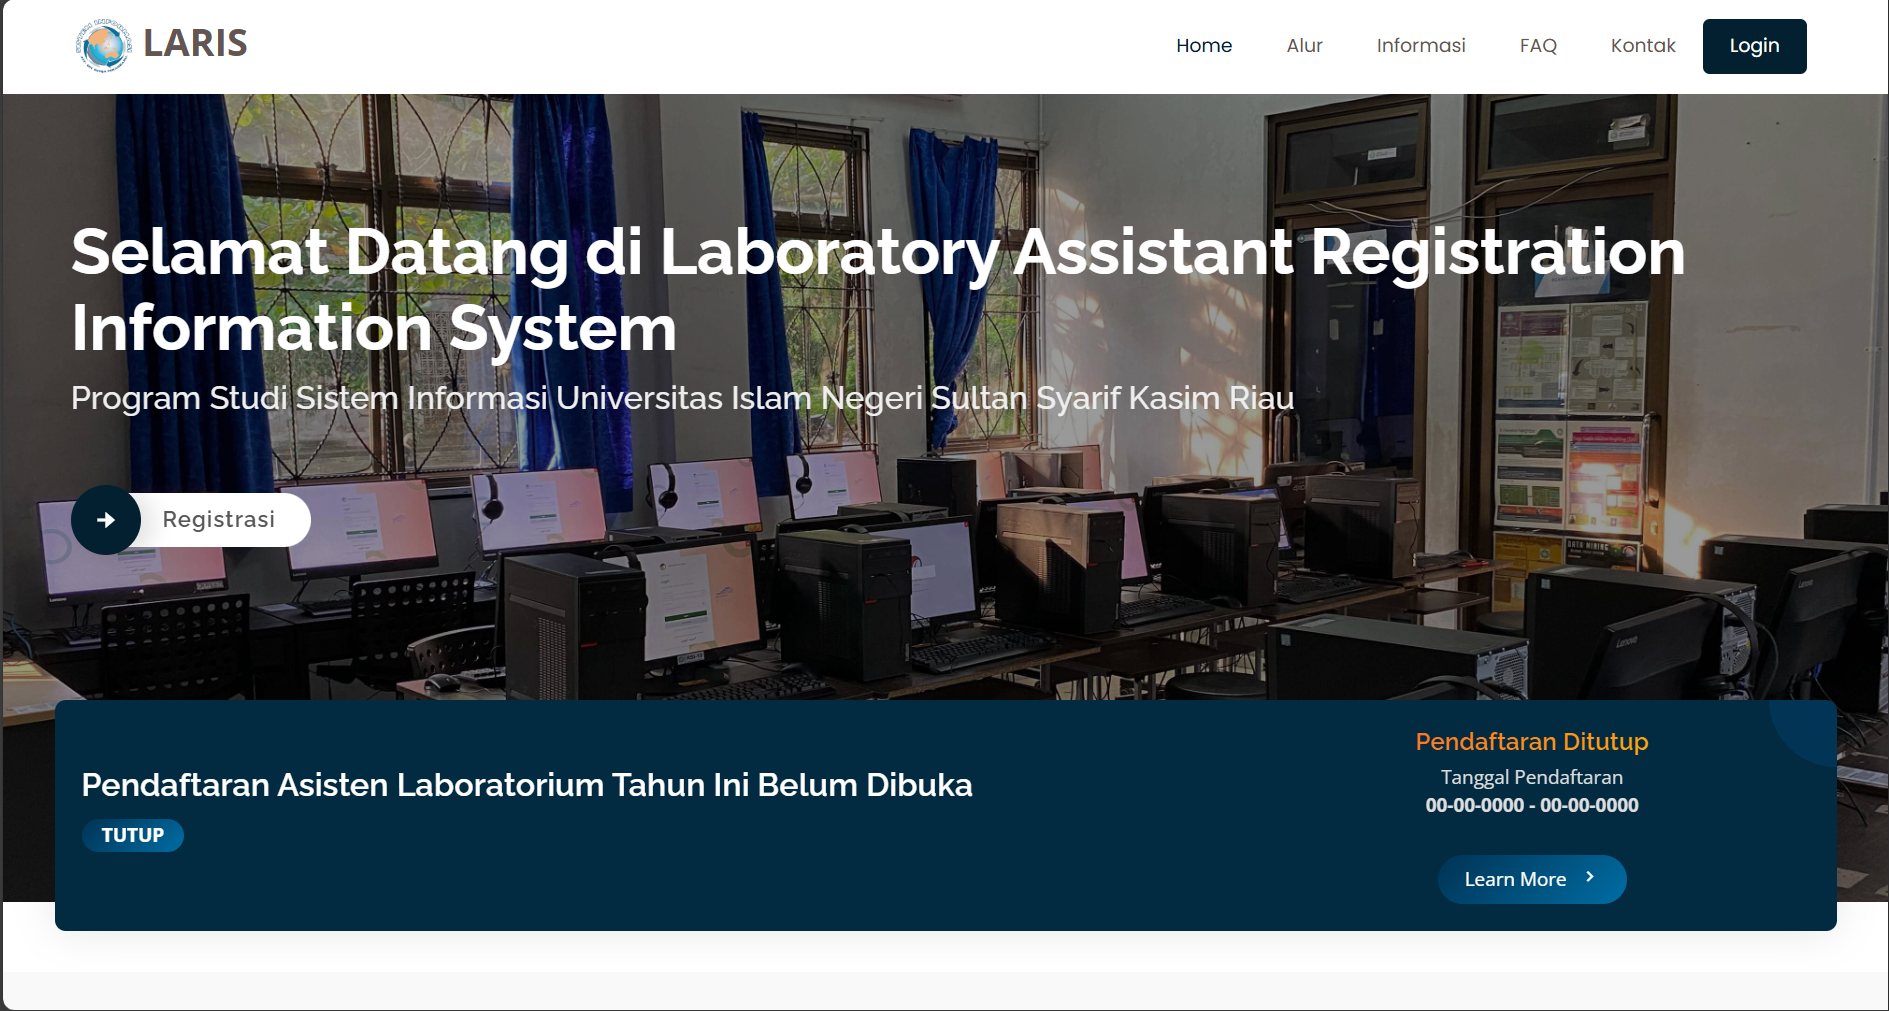
\includegraphics[width=0.82\linewidth]{konten//gambar/laris.png}
	\caption{\textit{Laboratory Assistant Registration Information System (LARIS)} \protect\cite{web-prodi}}
	\label{fig:laris}
\end{figure}

\section{SITARIS SI}
Sistem Informasi Inventaris Laboratorium adalah sebuah platform yang dibuat dengan menggunakan Framework CodeIgniter4 dan bahasa pemrograman PHP yang dimaksudkan untuk membantu mengelola dan memantau inventaris barang dan peralatan laboratorium. Sistem ini memiliki potensi untuk meningkatkan efisiensi dan produktivitas dalam operasional laboratorium berkat berbagai fitur utama yang ditawarkannya.

Dengan adanya sistem ini, diharapkan pengelolaan inventaris laboratorium menjadi lebih mudah dan efisien, sehingga staf laboratorium dapat fokus pada tugas yang lebih penting. Selain itu, laporan yang dihasilkan oleh sistem dapat membantu dalam pengambilan keputusan yang lebih baik tentang persediaan barang dan peralatan laboratorium \cite{sitaris-lab-si-website}. SITARIS SI dapat diakses di alamat https://sitaris.lab-si.uin-suska.ac.id. Terdapat beberapa menu yang ada pada SITARIS SI, yaitu:

\begin{enumerate}
	\item Halaman \textit{login} \\ Halaman \textit{login} merupakan tampilan awal sistem ketika diakses. Terdapat formulir \textit{username} dan \textit{password} dan dilindungi oleh anti spam dari google reCAPTCHA yang digunakan untuk masuk ke dalam sistem informasi inventaris seperti pada Gambar 2.2.

	      \begin{figure}
		      \centering
		      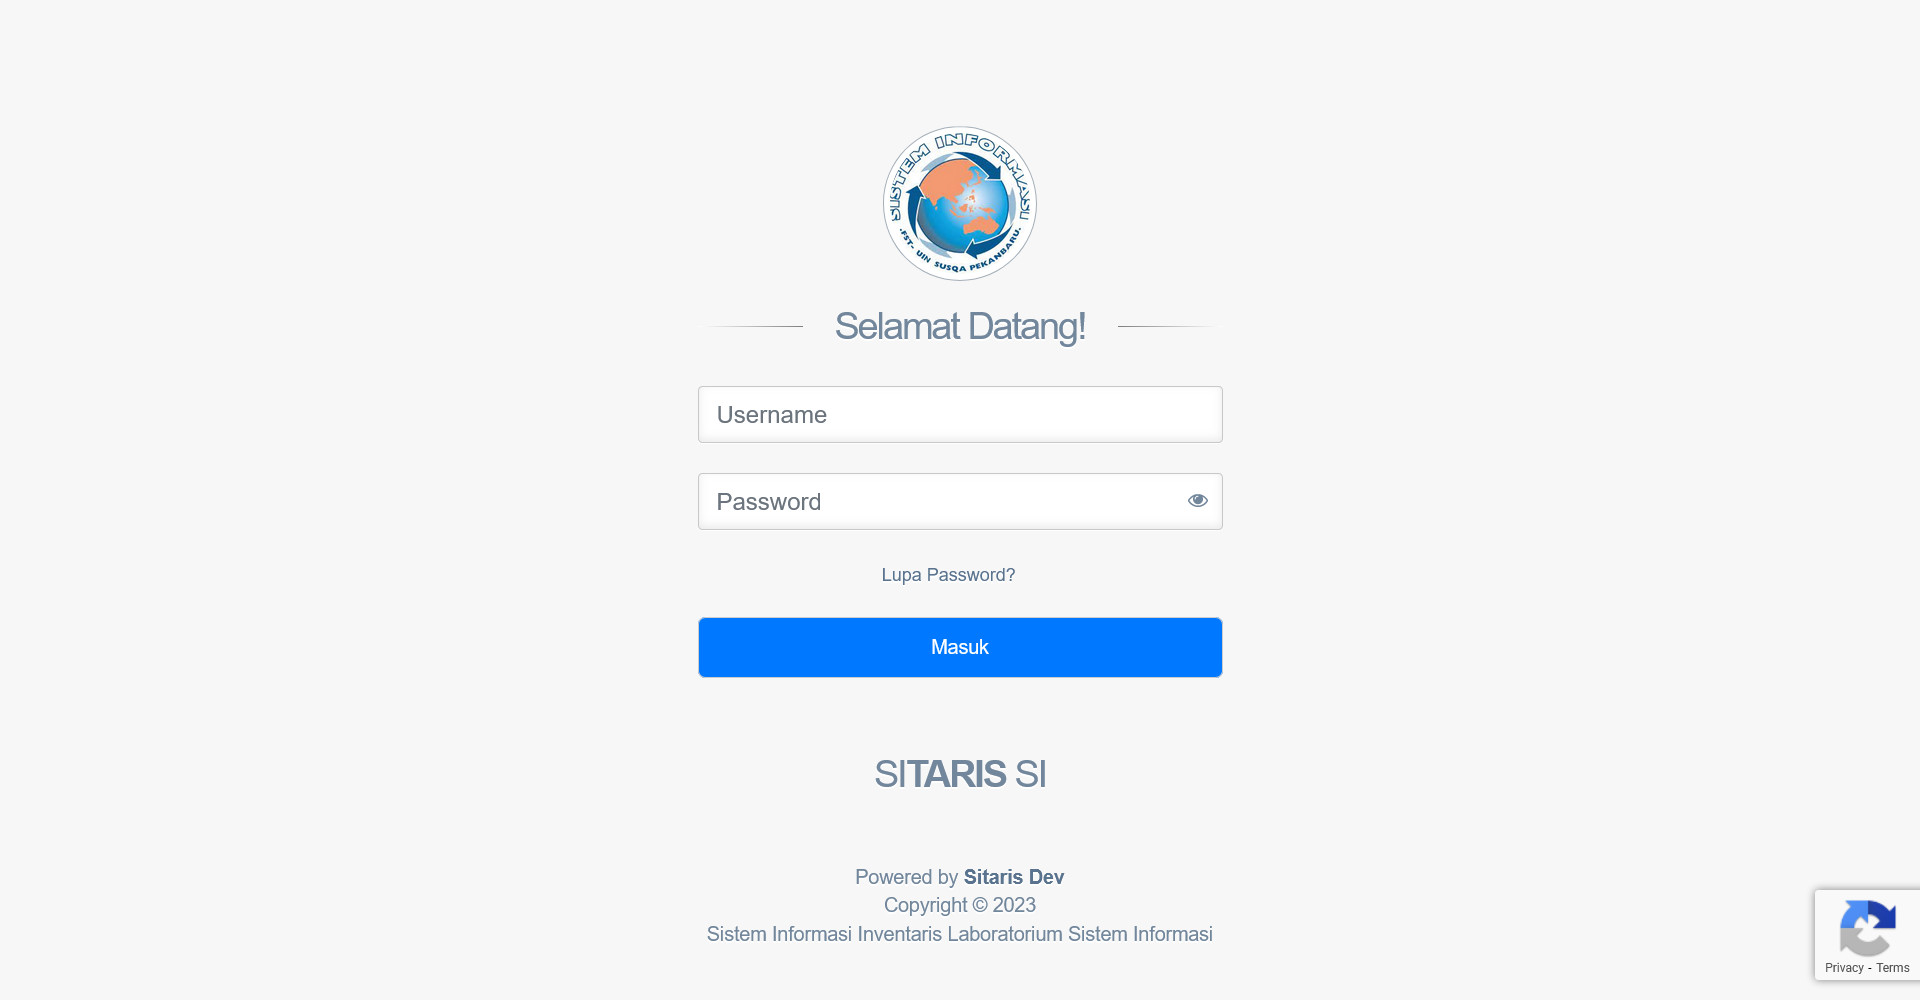
\includegraphics[width=0.82\linewidth]{konten//gambar/Login Page.png}
		      \caption{Halaman \textit{Login}}
		      \label{fig:sitaris}
	      \end{figure}

	\item Halaman Beranda \\ Halaman beranda merupakan tampilan awal yang ditampilkan kepada \textit{user} jika \textit{user} berhasil \textit{login} seperti pada Gambar 2.3.

	      \begin{figure}
		      \centering
		      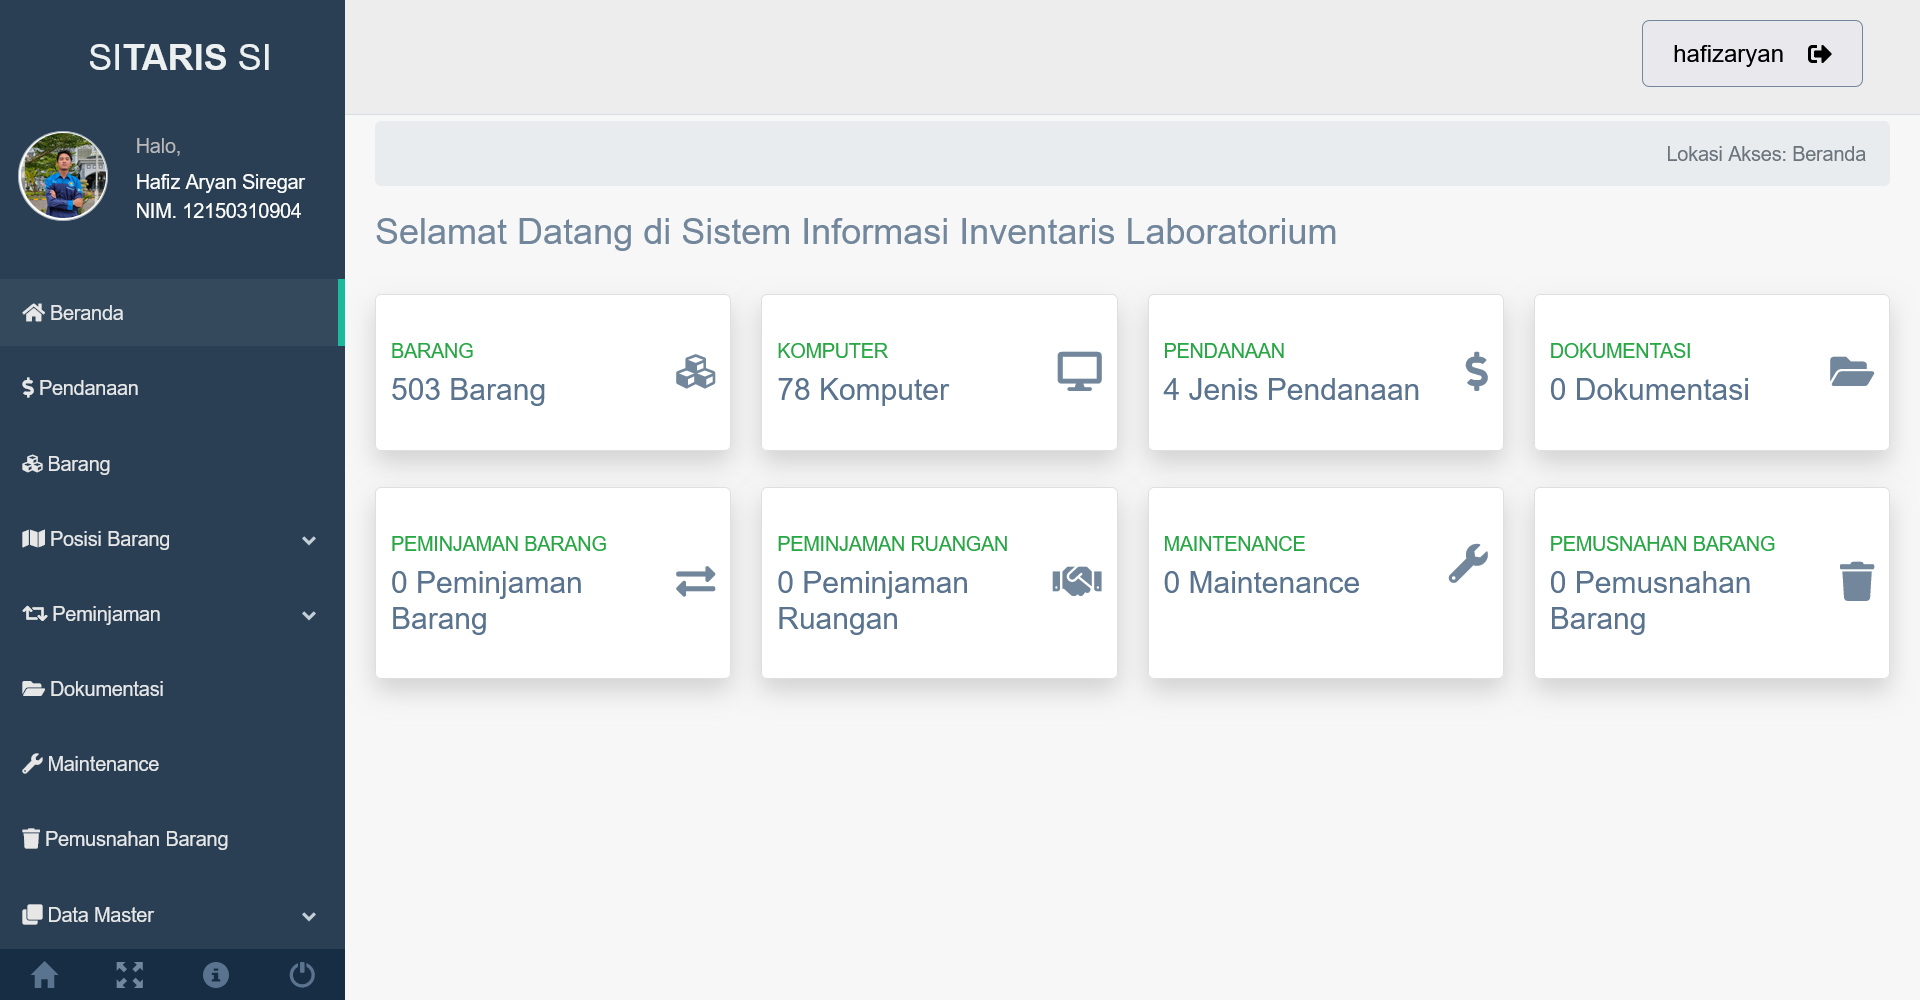
\includegraphics[width=0.82\linewidth]{konten//gambar/login berhasil.png}
		      \caption{Halaman Beranda}
		      \label{fig:enter-label}
	      \end{figure}

	\item Halaman Barang \\ Halaman barang merupakan tampilan untuk melihat dan mengelola data barang, tombol tambah data merupakan tombol yang dapat digunakan untuk beralih ke halaman tambah data barang, dan tombol pensil digunakan untuk mengedit data barang dan tombol \textit{trash} untuk menghapus data barang, lalu terdapat juga tombol berwarna biru toska yang dibedakan menjadi beberapa tombol yang bertujuan untuk mencetak dokumen laporan berdasarkan pendanaan, ruangan, kategori, tahun, dan QR seperti pada Gambar 2.7. sampai Gambar 2.19.

	      \begin{figure}
		      \centering
		      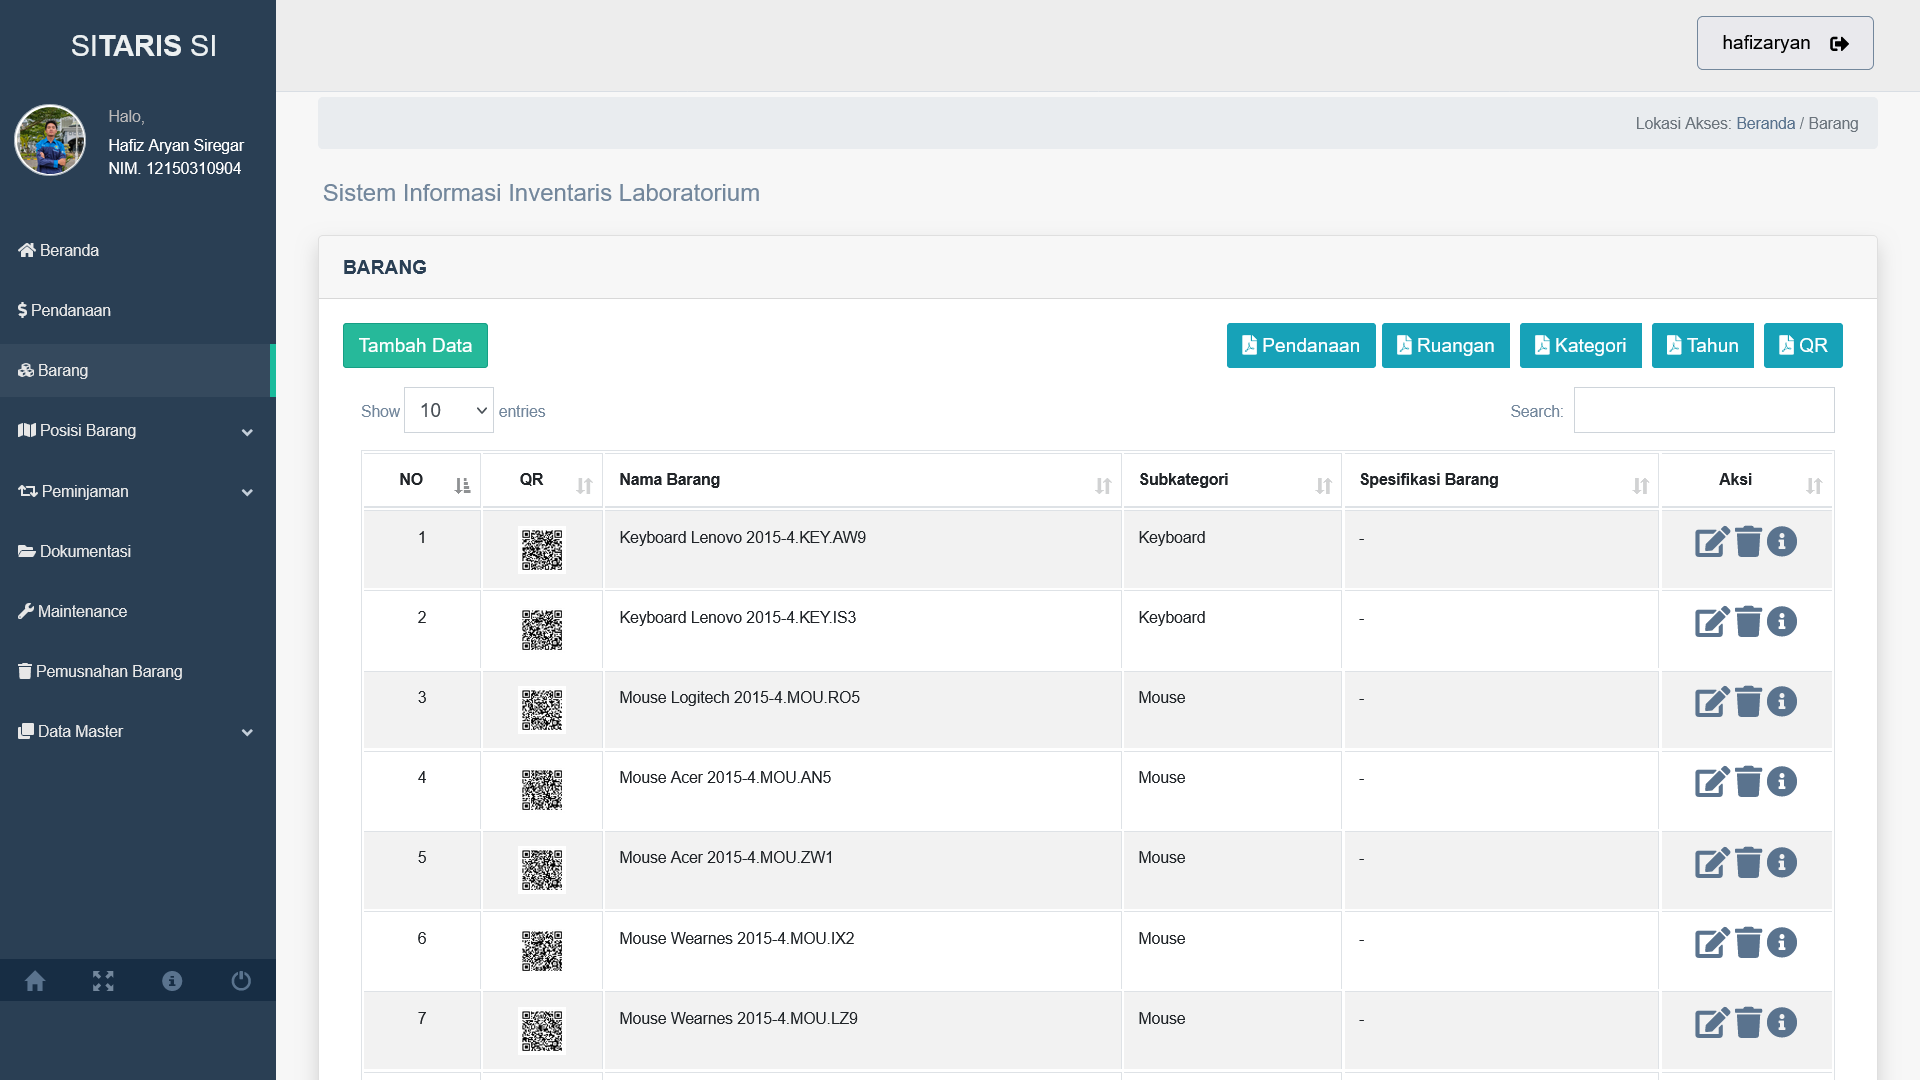
\includegraphics[width=0.82\linewidth]{konten//gambar/barang.png}
		      \caption{Halaman Barang \textit{Index}}
		      \label{fig:enter-label}
	      \end{figure}

\end{enumerate}

\section{Model Pengembangan Sistem}
Dalam penelitian ini, digunakan model pengembangan sistem Agile sebagai metodologi pengembangan perangkat lunak. Ada berbagai metode dan pendekatan pengembangan perangkat lunak tradisional seperti pendekatan waterfall, pendekatan iterative dan inkremental, pendekatan spiral, dan pendekatan evolutif. Pendekatan-pendekatan ini sering disebut sebagai pendekatan pengembangan perangkat lunak terencana atau pendekatan kelas berat. Pendekatan-pendekatan ini sangat berguna dalam mengembangkan perangkat lunak yang kompleks, membantu menghindari pengembangan perangkat lunak gaya lama yang informal dan memberikan perangkat lunak berkualitas tinggi secara sistematis, sehingga memenuhi persyaratan pengguna dalam batas waktu yang telah ditentukan \cite{al2020agile}.

\begin{figure}
	\centering
	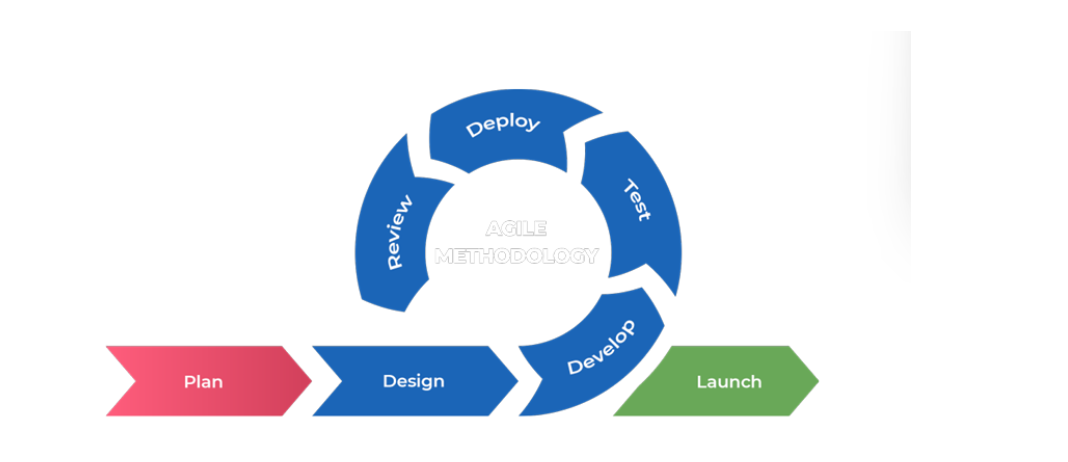
\includegraphics[width=0.82\linewidth]{konten//gambar/agile.png}
	\caption{\textit{Agile Development}}
	\label{fig:enter-label}
\end{figure}

\section{\textit{Unified Modelling Language} (UML)}

\textit{Unified Modelling Language} (UML) merupakan sebuah bahasa yang berdasarkan grafik/gambar untuk memvisualisasi, menspesifikasikan, membangun, dan pendokumentasian dari sebuah sistem pengembangan \textit{software}. UML sendiri juga memberikan standar penelitian sebuah sistem \textit{blue print}, yang meliputi konsep bisnis proses, penelitian kelas-kelas dalam bahasa program yang spesifik, skema \textit{database}, dan komponen-komponen yang diperlukan dalam sistem \textit{software} \cite{Mubarak2019}. Ada beberapa jenis diagram UML untuk membantu perancangan sistem antara lain:

\begin{enumerate}
	\item \textit{Use Case Diagram} \\
	      Menggambarkan fungsionalitas yang diharapakan dari sebuah sistem, dan merepresentasikan sebuah interaksi antara aktor dan sistem. Didalam \textit{use case} terdapat aktor sebagai gambaran entitas dari manusia atau sebuah sistem yang melakukan pekerjaan di sistem. Keterangan Simbol \textit{Use Case Diagram} dapat dilihat pada \tab~\ref{tab21}.

	      {
	      \fontsize{10}{12}\selectfont
	      \begin{longtable}{|c|c|c|l|}
		      \caption{Deskripsi \textit{Use Case Diagram}}
		      \label{tab21}                                                                                                                                                                                                                                                                                                                                                                \\
		      \hline
		      No & Simbol                                                                                                           & Nama                    & \multicolumn{1}{c|}{Keterangan}                                                                                                                                                                                            \\ \hline
		      \endfirsthead
		      %
		      \multicolumn{4}{c}{\tablename\ \thetable\ {Deskripsi \textit{Activity} Diagram} \space (Tabel lanjutan...)}                                                                                                                                                                                                                                                                  \\
		      \endhead
		      %
		      1  & \begin{tabular}[c]{@{}l@{}} 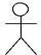
\includegraphics[height= 1.22cm, width= 0.91cm]{konten/gambar/uc1.jpg} \end{tabular} & \textit{Actor}          & \begin{tabular}[c]{@{}l@{}}Menspesifikasikan himpunan peran yang\\ pengguna mainkan ketika berinteraksi den-\\ gan use case.\end{tabular}                                                                                  \\ \hline
		      2  & \begin{tabular}[c]{@{}l@{}} 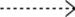
\includegraphics[height= 0.21cm, width= 0.91cm]{konten/gambar/uc2.png} \end{tabular} & \textit{Depedency}      & \begin{tabular}[c]{@{}l@{}}Hubungan dimana perubahan terjadi pada\\ suatu elemen yang mandiri (independent)\\ akan mempengaruhi elemen yang bergan-\\ tung padanya elemen yang tidak mandiri\\ (independent).\end{tabular} \\ \hline
		      3  & \begin{tabular}[c]{@{}l@{}} 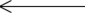
\includegraphics[height= 0.21cm, width= 0.91cm]{konten/gambar/uc3.png} \end{tabular} & \textit{Generelization} & \begin{tabular}[c]{@{}l@{}}Hubungan dimana objek anak (descendent)\\ berbagi prilaku dan struktur dari data objek\\ yang ada di atasnya objek induk (ancestor).\end{tabular}                                               \\ \hline
		      4  & \begin{tabular}[c]{@{}l@{}} 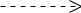
\includegraphics[height= 0.21cm, width= 0.91cm]{konten/gambar/uc4.png} \end{tabular} & \textit{Include}        & \begin{tabular}[c]{@{}l@{}}Menspesifikasikan bahwa use case sumber\\ secara eksplisit.\end{tabular}                                                                                                                        \\ \hline
		      5  & \begin{tabular}[c]{@{}l@{}} 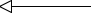
\includegraphics[height= 0.21cm, width= 0.91cm]{konten/gambar/uc5.png} \end{tabular} & \textit{Extend}         & \begin{tabular}[c]{@{}l@{}}Menspesifikasikan bahwa use case target\\ memperluas perilaku dari use case sumber\\ pada suatu titik yang diberikan.\end{tabular}                                                              \\ \hline
		      6  & \begin{tabular}[c]{@{}l@{}} 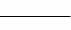
\includegraphics[height= 0.21cm, width= 0.91cm]{konten/gambar/uc6.png} \end{tabular} & \textit{Association}    & \begin{tabular}[c]{@{}l@{}}Apa yang menghubungkan antara objek satu\\ dengan objek lainnya.\end{tabular}                                                                                                                   \\ \hline
		      7  & \begin{tabular}[c]{@{}l@{}} 
\includegraphics[height= 1.42cm, width= 0.91cm]{konten/gambar/uc7.png} \end{tabular} & \textit{System}         & \begin{tabular}[c]{@{}l@{}}Menspesifikasikan paket yang menampilkan\\ sistem secara terbatas.\end{tabular}                                                                                                                 \\ \hline
		      8  & \begin{tabular}[c]{@{}l@{}} 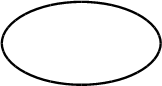
\includegraphics[height= 0.52cm, width= 0.98cm]{konten/gambar/uc8.png} \end{tabular} & \textit{Use Case}       & \begin{tabular}[c]{@{}l@{}}Deskripsi dari urutan aksi-aksi yang ditam-\\ pilkan sistem yang menghasilkan suatu hasil\\ yang terukur bagi suatu aktor.\end{tabular}                                                         \\ \hline
		      9  & \begin{tabular}[c]{@{}l@{}} 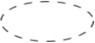
\includegraphics[height= 0.48cm, width= 1.06cm]{konten/gambar/uc9.jpg} \end{tabular} & \textit{Collaboration}  & \begin{tabular}[c]{@{}l@{}}Interaksi aturan-aturan dan elemen lain\\ yang bekerja sama untuk menyediakan per-\\ ilaku yang lebih bear dari jumlah dan\\ elemen-elemennya (sinergi).\end{tabular}                           \\ \hline
	      \end{longtable}
	      }

	\item \textit{Activity} Diagram \\
	      Diagram aktivitas atau \textit{Activity} diagram menggambarkan aliran fungsiona- liatas sistem. Pada tahap pemodelan bisnis, diagram aktivitas dapat digu- nakan untuk menunjukkan aliran kerja bisnis (\textit{businness work flow}). Da- pat juga digunakan untuk menggambarkan aliran kejadian (\textit{flow of event}) dalam \textit{use case}. Aktivitas menggambarkan proses yang berjalan, sementara \textit{use case} menggambarkan bagaiman aktor menggunakan sistem untuk melakukan aktivitas. Tabel Keterangan Simbol \textit{Activity} Diagram dapat dili- hat pada  \tab~\ref{tab22}.

	      {
	      \fontsize{10}{12}\selectfont
	      \begin{longtable}{|c|c|c|l|}
		      \caption{Deskripsi \textit{Activity Diagram}}
		      \label{tab22}                                                                                                                                                                                                                                                                     \\
		      \hline
		      No & Simbol                                                                                                           & Nama                    & \multicolumn{1}{c|}{Keterangan}                                                                                                 \\ \hline
		      \endfirsthead
		      %
		      \multicolumn{4}{c}{\tablename\ \thetable\ {Deskripsi \textit{Activity Diagram}} \space (Tabel lanjutan...)}                                                                                                                                                                       \\
		      \endhead
		      %
		      1  & \begin{tabular}[c]{@{}l@{}} 
\includegraphics[height= 0.51cm, width= 0.94cm]{konten/gambar/ac1.png} \end{tabular} & \textit{Activity}       & \begin{tabular}[c]{@{}l@{}}Memperlihatkan bagaimana masing- masing \\kelas antau antar muka saling berinteraksi\\satu sama lain.
		                                                                                                                                                        \end{tabular} \\ \hline
		      2  & \begin{tabular}[c]{@{}l@{}} 
\includegraphics[height= 0.47cm, width= 0.94cm]{konten/gambar/ac2.png} \end{tabular} & \textit{Action}         & \begin{tabular}[c]{@{}l@{}}State dari sistem yang mencerminkan\\eksekusi dari suatu aksi\end{tabular}                           \\ \hline
		      3  & \begin{tabular}[c]{@{}l@{}} 
\includegraphics[height= 0.6cm, width= 0.6cm]{konten/gambar/ac3.png} \end{tabular}   & \textit{Initial node}   & Bagaimana objek dibentuk atau diawali.                                                                                          \\ \hline
		      4  & \begin{tabular}[c]{@{}l@{}} 
\includegraphics[height= 0.6cm, width= 0.6cm]{konten/gambar/ac4.png} \end{tabular}   & \textit{Activity final} & Bagaimana objek dibentuk dan dihancurkan                                                                                        \\ \hline
		      5  & \begin{tabular}[c]{@{}l@{}} 
\includegraphics[height= 0.06cm, width= 0.94cm]{konten/gambar/ac5.png} \end{tabular} & \textit{Fork node}      & \begin{tabular}[c]{@{}l@{}}Satu aliran yang pada tahap tertentu berubah\\ menjadi beberapa aliran.\end{tabular}                 \\ \hline
	      \end{longtable}
	      }

	\item Class  Diagram \\
	      \textit{Class Diagram} menggambarkan struktur statis dari kelas dalam sistem dan menggambarkan atribut, operasi dan hubungan antara kelas. \textit{Class Diagram} juga membantu dalam memvisualisasikan struktur kelas-kelas dari suatu sis- tem dan merupakan tipe diagram yang paling banyak dipakai. Keterangan Simbol \textit{Class Diagram} dapat dilihat pada  \tab~\ref{tab23}.

	      {
	      \fontsize{10}{12}\selectfont
	      \begin{longtable}{|c|c|c|l|}
		      \caption{Deskripsi \textit{Class Diagram}}
		      \label{tab23}                                                                                                                                                                                                                                                                                                                                                          \\
		      \hline
		      No & Simbol                                                                                                           & Nama                                                                                      & \multicolumn{1}{c|}{Keterangan}                                                                                                                    \\ \hline
		      \endfirsthead
		      %
		      \multicolumn{4}{c}{\tablename\ \thetable\ {Deskripsi \textit{Class Diagram}} \space (Tabel lanjutan...)}                                                                                                                                                                                                                                                               \\
		      \endhead
		      %
		      1  & \begin{tabular}[c]{@{}l@{}} 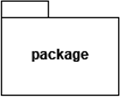
\includegraphics[height= 0.8cm, width= 0.98cm]{konten/gambar/cd1.png} \end{tabular}  & \textit{Package}                                                                          & \begin{tabular}[c]{@{}l@{}}\textit{Package} merupakan sebuah bungku- \\san dari satu atau lebih kelas.
		                                                                                                                                                                                                                          \end{tabular}                                              \\ \hline
		      2  & \begin{tabular}[c]{@{}l@{}} 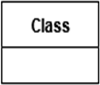
\includegraphics[height= 0.61cm, width= 0.71cm]{konten/gambar/cd2.png} \end{tabular} & Operasi                                                                                   & Kelas pada struktur sistem.                                                                                                                        \\ \hline
		      3  & \begin{tabular}[c]{@{}l@{}} 
\includegraphics[height= 0.22cm, width= 1.05cm]{konten/gambar/cd3.png} \end{tabular} & \begin{tabular}[c]{@{}c@{}} Asosiasi berarah/\\\textit{Directed asociation} \end{tabular} & \begin{tabular}[c]{@{}l@{}} Relasi antar kelas dengan makna u-\\mum, asosiasi biasanya juga disertai\\ dengan \textit{multiplicity}. \end{tabular} \\ \hline
		      4  & \begin{tabular}[c]{@{}l@{}} 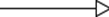
\includegraphics[height= 0.22cm, width= 1.05cm]{konten/gambar/cd4.png} \end{tabular} & \textit{Generalisasi}                                                                     & \begin{tabular}[c]{@{}l@{}} Relasi antar kelas dengan mak \\na generalisasi spesialisasi (umum\\khusus). \end{tabular}                             \\ \hline
		      5  & \begin{tabular}[c]{@{}l@{}} 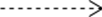
\includegraphics[height= 0.22cm, width= 1.05cm]{konten/gambar/cd5.png} \end{tabular} & \begin{tabular}[c]{@{}c@{}}Kebergantungan/\\\textit{Defedency}\end{tabular}               & \begin{tabular}[c]{@{}l@{}}Relasi antar kelas dengan makna ke-\\bergantungan antar kelas.\end{tabular}                                             \\ \hline
	      \end{longtable}
	      }

\end{enumerate}

\section{Observasi}
Observasi adalah tindakan mengamati secara langsung perilaku individu, objek, atau aktivitas dengan cara yang teratur tanpa melakukan interaksi lansung dengan subjek yang diamati. Observasi merupakan metode pengumpulan data di mana pengamat mengamati suatu sistem atau entitas saat sedang beroperasi untuk mendapatkan wawasan dan pemahaman yang lebih mendalam tentang bagaimana sistem tersebut bekerja \cite{tilley2017systems}.

\section{Wawancara}
Wawancara adalah metode pengumpulan data yang dilakukan melalui tanya jawab langsung antara peneliti dengan narasumber atau responden untuk mendapatkan informasi yang dibutuhkan \cite{monday2020impacts}. Teknik ini memungkinkan peneliti untuk mengumpulkan data kualitatif yang mendalam dan memahami perspektif, pengalaman, serta pengetahuan dari narasumber secara langsung. Wawancara dapat dilakukan secara terstruktur dengan menggunakan daftar pertanyaan yang telah disiapkan sebelumnya, semi-terstruktur yang memungkinkan fleksibilitas dalam mengajukan pertanyaan, atau tidak terstruktur yang bersifat lebih informal dan mengalir \cite{balza2022effective}. Dalam konteks pengembangan sistem, wawancara sering digunakan untuk mengidentifikasi kebutuhan pengguna, mengumpulkan persyaratan sistem, dan memahami proses bisnis yang ada \cite{rueda2020requirements}.

\section{PHP}
PHP (PHP: Hypertext Preprocessor) adalah bahasa pemrograman server-side yang digunakan untuk membuat situs web dinamis dan interaktif. PHP merupakan bahasa pemrograman yang populer dan mudah dipelajari, serta memiliki banyak fungsi yang dapat digunakan untuk membuat situs web yang interaktif dan dinamis. PHP dapat digunakan untuk membuat situs web yang interaktif, seperti form pendaftaran, login, dan lainnya. PHP juga dapat digunakan untuk membuat situs web yang dinamis, seperti situs web yang dapat menampilkan data dinamis dari database \cite{irawan2017implementasi}.

% \begin{figure}
% 	\centering
% 	
\includegraphics[width=0.30\linewidth]{konten//gambar/logo-php.png}
% 	\caption{Logo PHP}
% 	\label{fig:enter-label}
% \end{figure}

\section{Framework}
\textit{Framework} dalam pengembangan sistem adalah kerangka kerja atau struktur yang digunakan untuk memudahkan pengembangan aplikasi atau sistem \cite{sallaby2020perancangan}. \textit{Framework} menyediakan berbagai fitur dan fungsi yang dapat digunakan oleh pengembang untuk mempercepat proses pengembangan dan memastikan konsistensi dalam pengembangan aplikasi atau sistem \cite{simanullang2021sistem}. \textit{Framework} juga membantu pengembang dalam mengelola kode program dan memperbaiki \textit{bug}. Beberapa contoh \textit{framework} yang sering digunakan dalam pengembangan sistem adalah Laravel, CodeIgniter, dan beberapa \textit{framework} lainnya \cite{Fadllullah2022PengembanganSI}.

\section{CodeIgniter}
Codeigniter merupakan \textit{framework} untuk membangun aplikasi \textit{web} berbasis PHP. Codeigniter menyediakan banyak \textit{library} untuk fungsi-fungsi umum, antar muka yang sederhana, dan struktur yang logis. CodeIgniter menjadi sebuah \textit{framework} PHP dengan model MVC (Model, View, Controller) untuk membangun \textit{website} dinamis dengan menggunakan PHP yang dapat mempercepat pengembang untuk membuat sebuah aplikasi \textit{web}. Selain ringan dan cepat, CodeIgniter juga memiliki dokumentasi yang super lengkap disertai dengan contoh implementasi kode-nya. \textit{Programmer} dapat membuat aplikasi dengan lebih cepat karena tidak perlu menulis kode dari awal, selain itu Codeigniter juga menyediakan banyak fungsi yang siap digunakan. Seorang \textit{programmer} bisa lebih fokus dengan aplikasi yang sedang dibangun dan meminimalkan penulisan kode \cite{tyowati2017implementasi}.

% \begin{figure}
% 	\centering
% 	
\includegraphics[width=0.20\linewidth]{konten//gambar/logo-codeigniter.png}
% 	\caption{Logo CodeIgniter}
% 	\label{fig:enter-label}
% \end{figure}

\section{\textit{Black Box} Testing}
\textit{Black Box Testing} adalah metode pengujian perangkat lunak yang berfokus pada fungsionalitas eksternal sistem tanpa memperhatikan struktur internal kode. Dalam pengujian ini, pengujian dilakukan berdasarkan spesifikasi fungsional sistem dan tidak memerlukan pengetahuan tentang implementasi internal sistem \cite{ahsyar2021sistem}.

Metode \textit{Black Box Testing} dilakukan dengan cara menguji sistem dari luar, seperti pengguna akhir akan melakukannya. Pengujian ini bertujuan untuk memastikan bahwa sistem berfungsi sesuai dengan kebutuhan pengguna dan spesifikasi fungsional yang telah ditentukan.

\section{Visual Studio Code}
Visual Studio Code (VS Code) adalah editor kode serbaguna yang telah berkembang secara signifikan untuk mendukung berbagai lingkungan pemrograman di Windows, macOS, dan Linux. Ini mengintegrasikan fitur untuk menulis dan men-debug kode, termasuk dukungan untuk.NET 7 dan konsumsi layanan AI, meningkatkan produktivitas dan efisiensi pengembang \cite{bree2016using}

% \begin{figure}
% 	\centering
% 	
\includegraphics[width=0.30\linewidth]{konten//gambar/logo-vs-code.png}
% 	\caption{Logo Visual Studio Code}
% 	\label{fig:enter-label}
% \end{figure}

\section{Astah}
Astah adalah perangkat lunak pemodelan UML yang digunakan untuk merancang dan mendokumentasikan sistem perangkat lunak. Astah menyediakan berbagai fitur untuk membuat berbagai jenis diagram UML, seperti \textit{use case diagram, class diagram,} dan \textit{activity diagram} \cite{hayati2021sistem}. Peneliti menggunakan astah versi 10.0.0 untuk merancang pemodelan sistem ILMIS.
% \begin{figure}
% 	\centering
% 	
\includegraphics[width=0.3\textwidth]{konten/gambar/astah.png}
% 	\caption{Logo Astah}
% 	\label{LogoAstah}
% \end{figure}

\section{Balsamiq}
Balsamiq adalah perangkat lunak prototyping \textit{wireframing} yang digunakan untuk membuat desain awal aplikasi web dan mobile. Balsamiq menyediakan berbagai komponen UI yang siap pakai, seperti tombol, formulir, dan tabel, yang memungkinkan pengembang untuk membuat prototipe dengan cepat dan mudah. Balsamiq juga mendukung kolaborasi tim dan integrasi dengan berbagai alat pengembangan \cite{balsamiq}. Pada perancangan interface ini, versi balsamiq yang digunakan adalah versi 4.7.5.
% \begin{figure}
% 	\centering
% 	
\includegraphics[width=0.3\textwidth]{konten/gambar/balsamiq.jpg}
% 	\caption{Logo Balsamiq}
% 	\label{Balsamiq}
% \end{figure}

\section{\textit{Database}}
\textit{Database} adalah suatu kumpulan data yang telah diatur secara terstruktur, memungkinkan akses dan pengelolaan melalui sistem komputer. Jenis data yang dapat disimpan di dalamnya mencakup teks, gambar, suara, dan video, dengan berbagai tujuan seperti penyimpanan informasi, analisis data, dan pengambilan keputusan. Untuk membuat dan mengelola \textit{database}, diperlukan perangkat lunak khusus seperti \textit{MariaDB}, \textit{Oracle}, atau \textit{Microsoft SQL Server} \cite{Cowls2021ADB}.

\section{MariaDB}
MariaDB adalah sistem manajemen basis data relasional (RDBMS) yang dapat dijalankan di server web. MariaDB adalah versi terbaru dari MySQL, yang merupakan sistem manajemen basis data relasional (RDBMS) yang populer untuk aplikasi web. MariaDB memiliki fitur yang mirip dengan MySQL, tetapi memiliki beberapa perbedaan dalam implementasi dan performa. MariaDB juga memiliki dokumentasi yang lengkap dan dukungan komunitas yang kuat, sehingga memudahkan pengembang untuk membuat dan mengembangkan aplikasi web yang berjalan di server MariaDB \cite{mariadb2024}.

% \begin{figure}
% 	\centering
% 	
\includegraphics[width=0.20\linewidth]{konten//gambar/logo-mariadb.png}
% 	\caption{Logo MariaDB}
% 	\label{fig:enter-label}
% \end{figure}

\section{XAMPP}
XAMPP adalah sebuah paket lengkap untuk server web yang dapat dengan mudah diinstal di berbagai sistem operasi. Dalam paket ini sudah termasuk beberapa komponen penting seperti Apache (web server), MariaDB (database), PHP (server side scripting), dan berbagai pustaka pendukung lainnya. XAMPP dapat digunakan pada berbagai sistem operasi, termasuk Linux, Windows, MacOS, dan Solaris, sehingga memudahkan pembuatan server web multi-platform \cite{pakpahan2020sistem}.

% \begin{figure}
% 	\centering
% 	
\includegraphics[width=0.20\linewidth]{konten//gambar/logo-xampp.png}
% 	\caption{Logo XAMPP}
% 	\label{fig:enter-label}
% \end{figure}